\section{Reaching with an Obstacle}\label{sec:reach-obs}
Circling back to reaching, I introduced an obstacle placing mechanism as well as randomly placing the target behind this obstacle, ensuring the agent doesn't learn where exactly target is by looking at just the obstacle\todo[color=purple]. See Figure \ref{fig:reach-obs-random} for how this task looks and the check \todo[color=green]{add appendix link, and code} for the backend wiring of the task.

\subsection{Task}\label{subsec:ro-creating-the-task}
There are two versions of this task, I thought it might be interesting to randomise the object firstly dependently then independently on the obstacle. The `dependent' randomisation called \verb|ReachObs_Random| samples the obstacle, which in turn controls the spawn boundary of where the target can spawn in, meaning the target will always appear behind the obstacle albeit, edges of it can sometimes stick out. Conversely, the `independently' random version, called \verb|ReachObs_IndRandom|\todo[color=green]{also add to appendix and link here}, keeps the target spawn boundary fixed, meaning the target can be anywhere in the visible workspace, but it is not necessarily always covered by the obstacle. I can see that this potentially can be useful to keep the dataset a bit more diverse, and allow the wrist camera initially observe the target sometimes.\todo[color=red]{use this somewhere, or hint back to it, maybe even to say there was no difference}

\begin{figure}[htpb] % htpb allows all placement
  \centering
  \begin{subfigure}{0.3\linewidth}
    \centering
    \includegraphics[scale=0.3]{../fyp/assets/task-pics/reach-obs/random-front.png}
    \caption{Front}
  \end{subfigure}
  \hfill
  \begin{subfigure}{0.3\linewidth}
    \centering
    \includegraphics[scale=0.3]{../fyp/assets/task-pics/reach-obs/random-side.png}
    \caption{Side (Left)}
  \end{subfigure}
  \hfill
  \begin{subfigure}{0.3\linewidth}
    \centering
    \includegraphics[scale=0.3]{../fyp/assets/task-pics/reach-obs/random-top.png}
    \caption{Top}
  \end{subfigure}
  \vfill
  \begin{subfigure}{0.45\linewidth}
    \centering
    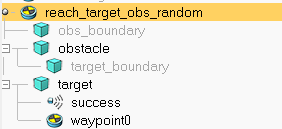
\includegraphics[scale=0.5]{assets/early-work/obs-random-scene-hierarchy.png}
    \caption{`ReachObs\_Random' Scene Hierarchy}
  \end{subfigure}
  \hfill
  \begin{subfigure}{0.45\linewidth}
    \centering
    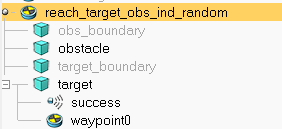
\includegraphics[scale=0.5]{assets/early-work/obs-ind-random-scene-hierarchy.png}
    \caption{`ReachObs\_IndRandom' Scene Hierarchy}
  \end{subfigure}
  \caption{Reaching Task with an Obstacle}\label{fig:reach-obs-random}
\end{figure}\todo[color=blue]{smaller?} 

\subsection{Running the Task}
There were a few interesting things of note happening on this task. 

I used the unchanged reaching policy from earlier\todo[color=green]{ref}. Unsurprisingly this did not perform amazingly, however, there are some important lessons to learn form what we are seeing here. Firstly, I adopted to observe the `minimum distance' to target this time \ref{subfig:ro-random-demo-mindist-10}, however the `final distance ' graph can be found in the appendix \todo[color=green]{link appendix}. 

\subsubsection{Why is `IndRandom' just worse?}
The experiments \todo[color=green]{appendix}, show that the `distance' graphs are translated upwards by roughly $0.1$m while the success rate is halved.

While they were trained on demos for their respective generation methods.They were evaluated using a shared a test set created using just \textbf{ReachObs\_Random}. This was a decision to be able to compare their results with each other and evaluate the differences of spawning techniques

This means that a policy trained on the independent generation is not as good at reaching the target successfully as often, but still manages to learn to get around the obstacle. Which tracks, as the independent task is easier, and predictions on a harder test set are tougher to fit.
This is likely due to to saved training demos for independent spawning being less occluded from the start. Training and testing the on the demos belonging to this task \ref{fig:ro-indrandom-demo-cams}, the results look a lot similar to what we expect from this model.


\begin{figure}[htpb] % htpb allows all placement
  \centering
  \begin{subfigure}{0.45\linewidth}
    \centering
    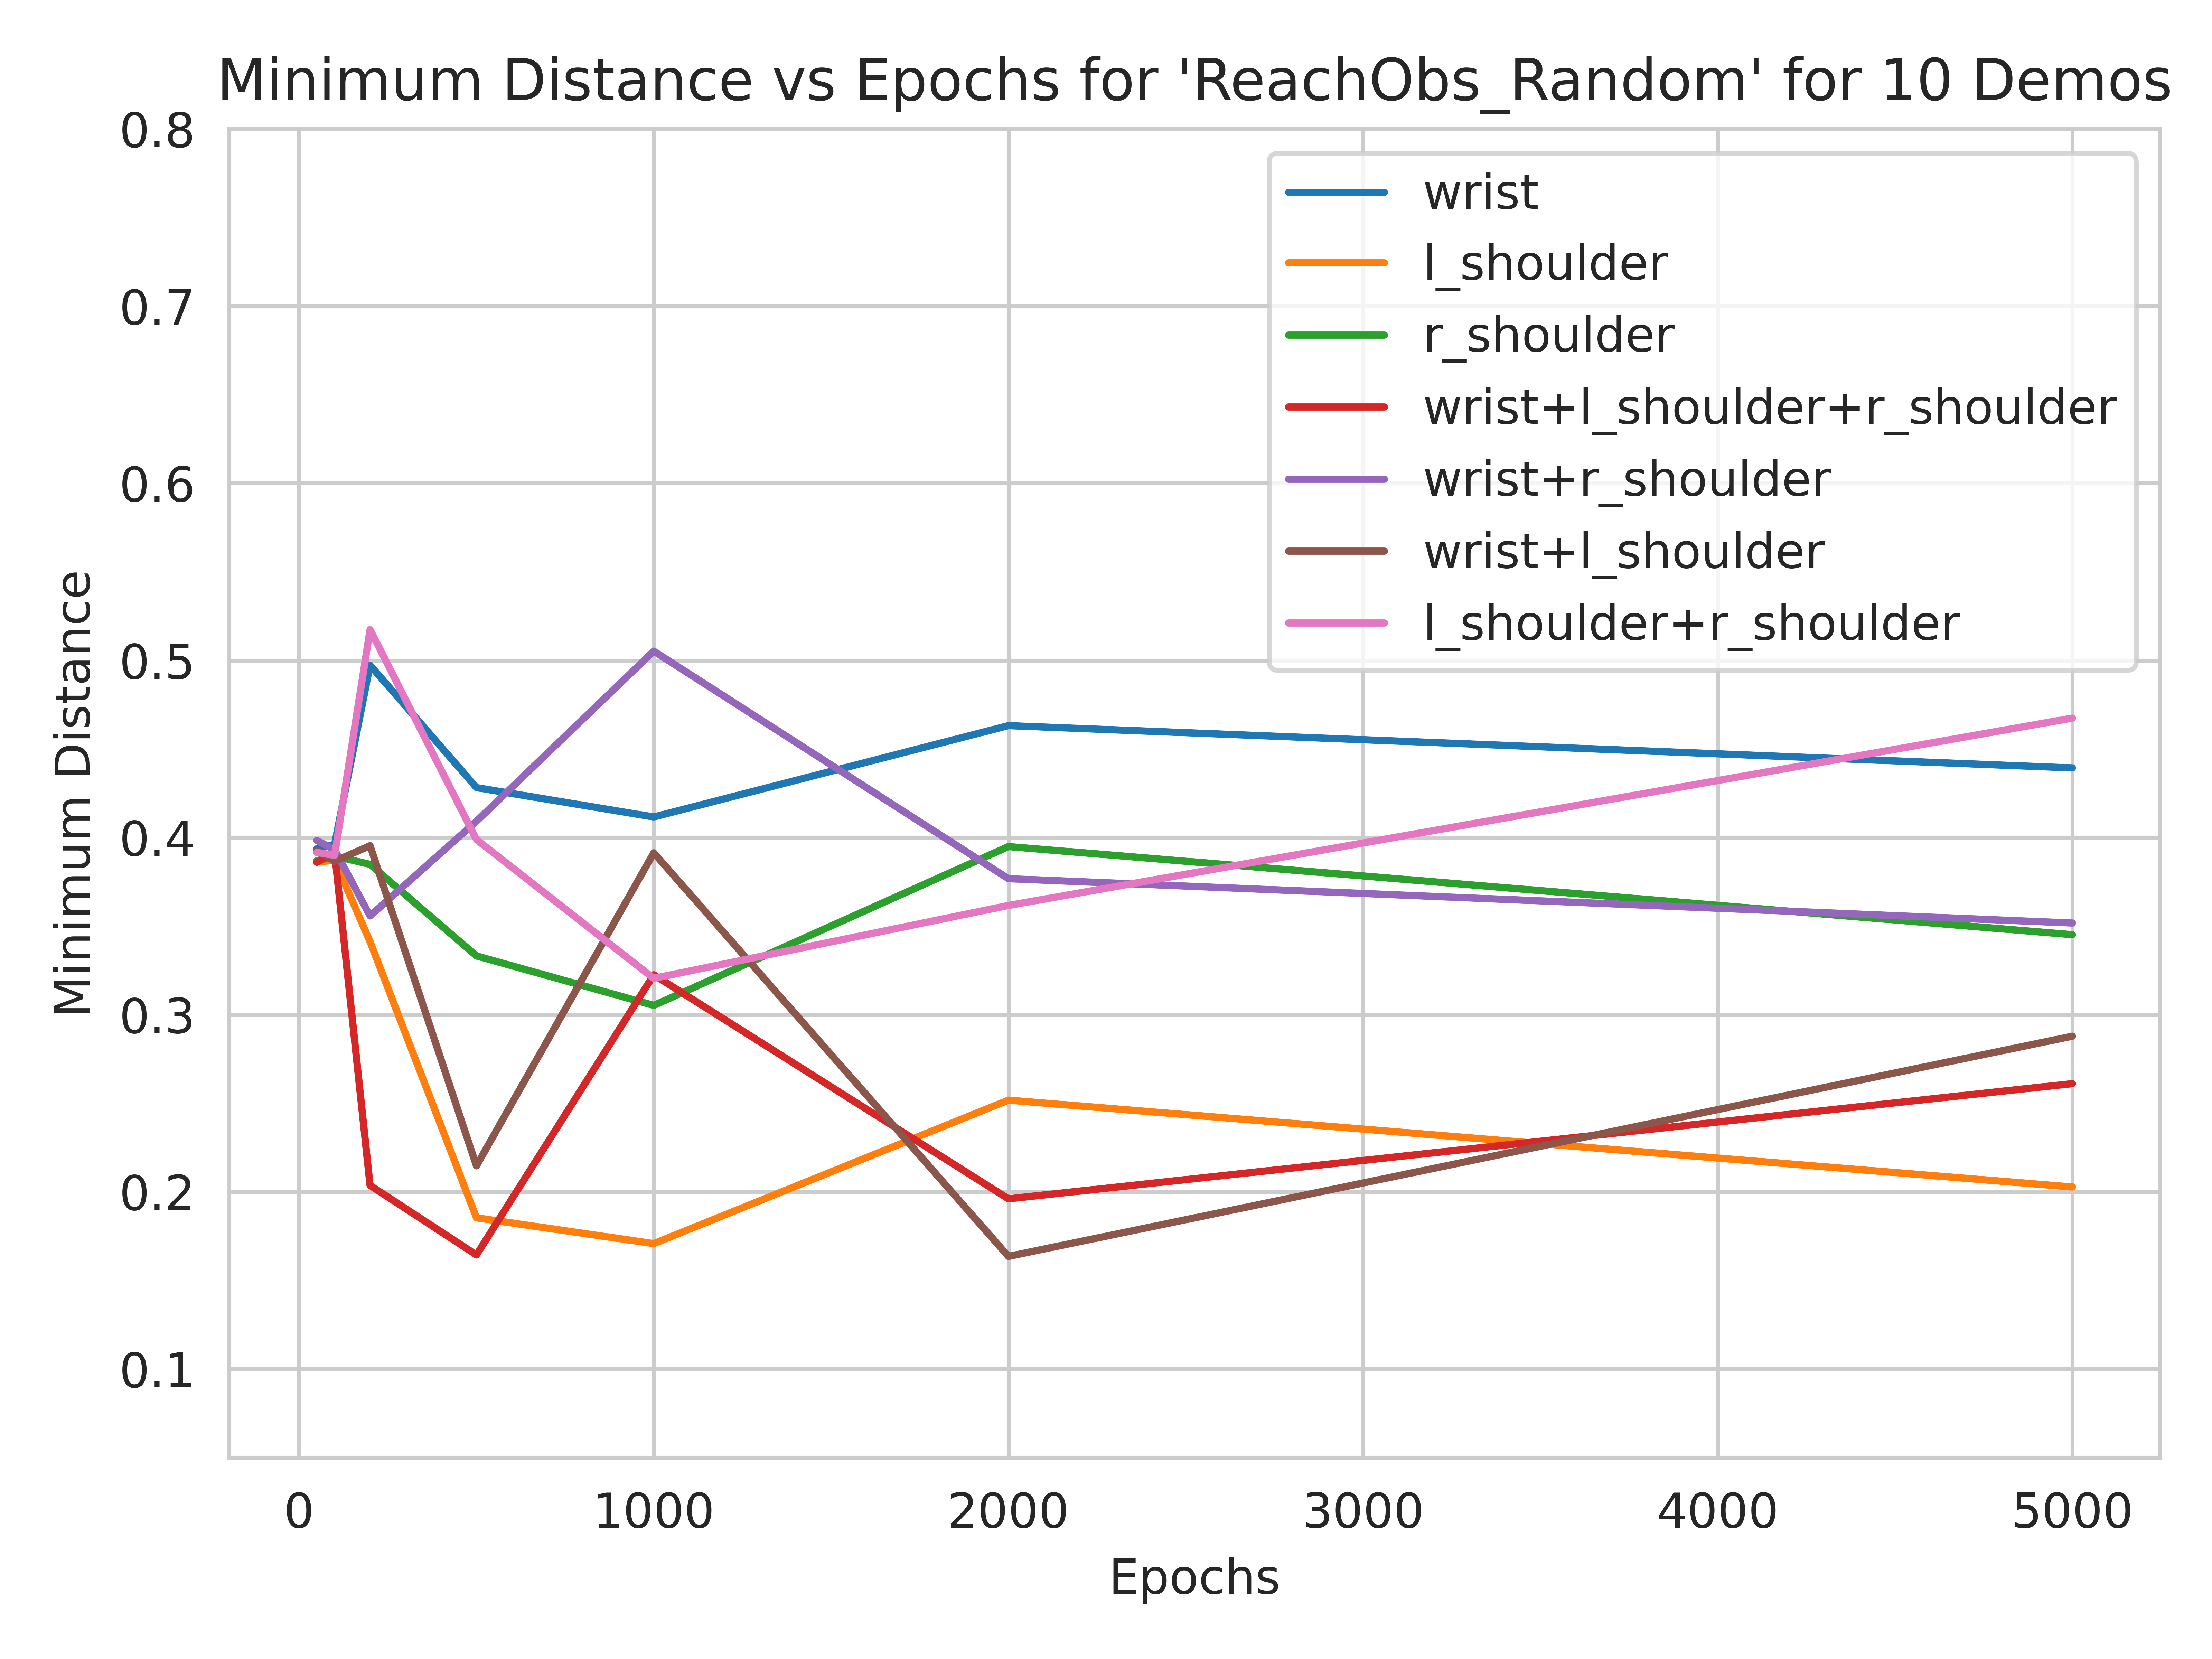
\includegraphics[width=\linewidth]{assets/cam-comb/reach-obs/ro_random-demo-mindist-10demos.png}
    \caption{Minimum Distance to Target}\label{subfig:ro-random-demo-mindist-10}
  \end{subfigure}
  \begin{subfigure}{0.45\linewidth}
    \centering
    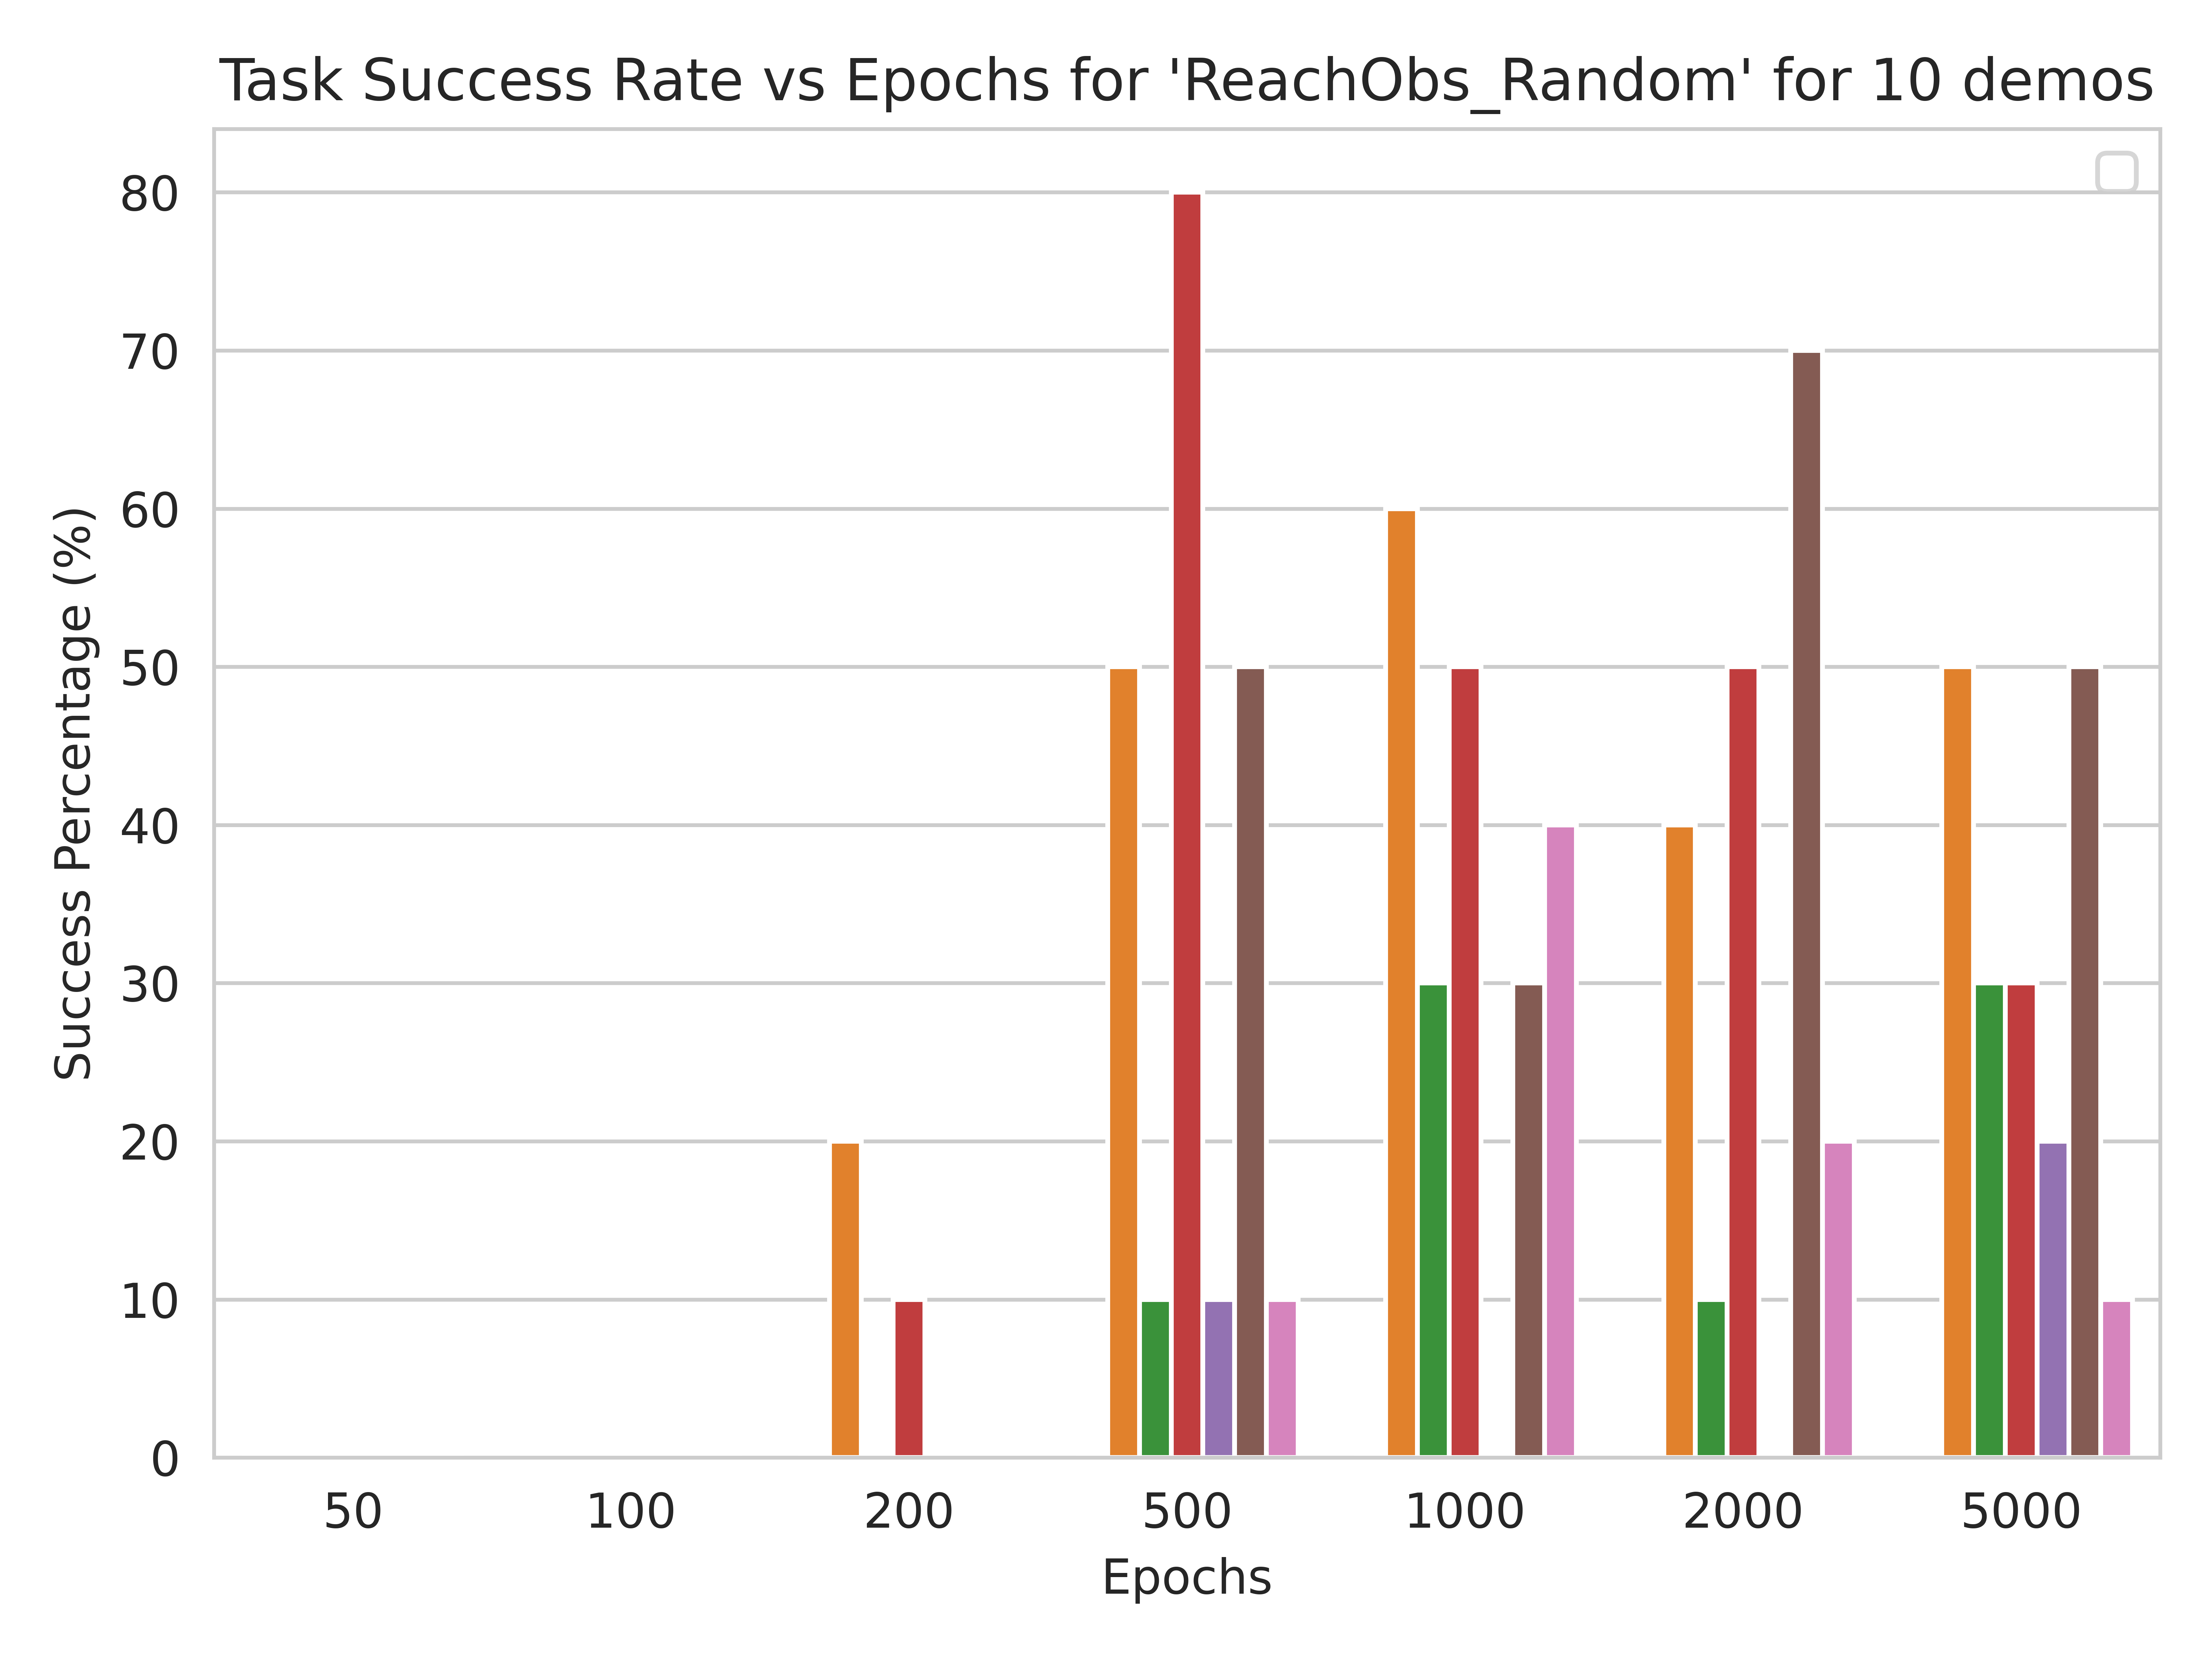
\includegraphics[width=\linewidth]{assets/cam-comb/reach-obs/ro_random-demo-success-10demos.png}
    \caption{Success Rate (\%) of Task}\label{subfig:ro-random-demo-success-10}
  \end{subfigure}
  \caption{Policy trained on 10 demos, using the \emph{demo dataset} from \ref{subsec:grasp-data-loading-changes}}\label{fig:ro-random-demo-cams}
\end{figure}

\begin{figure}[htpb] % htpb allows all placement
  \centering
  \begin{subfigure}{0.45\linewidth}
    \centering
    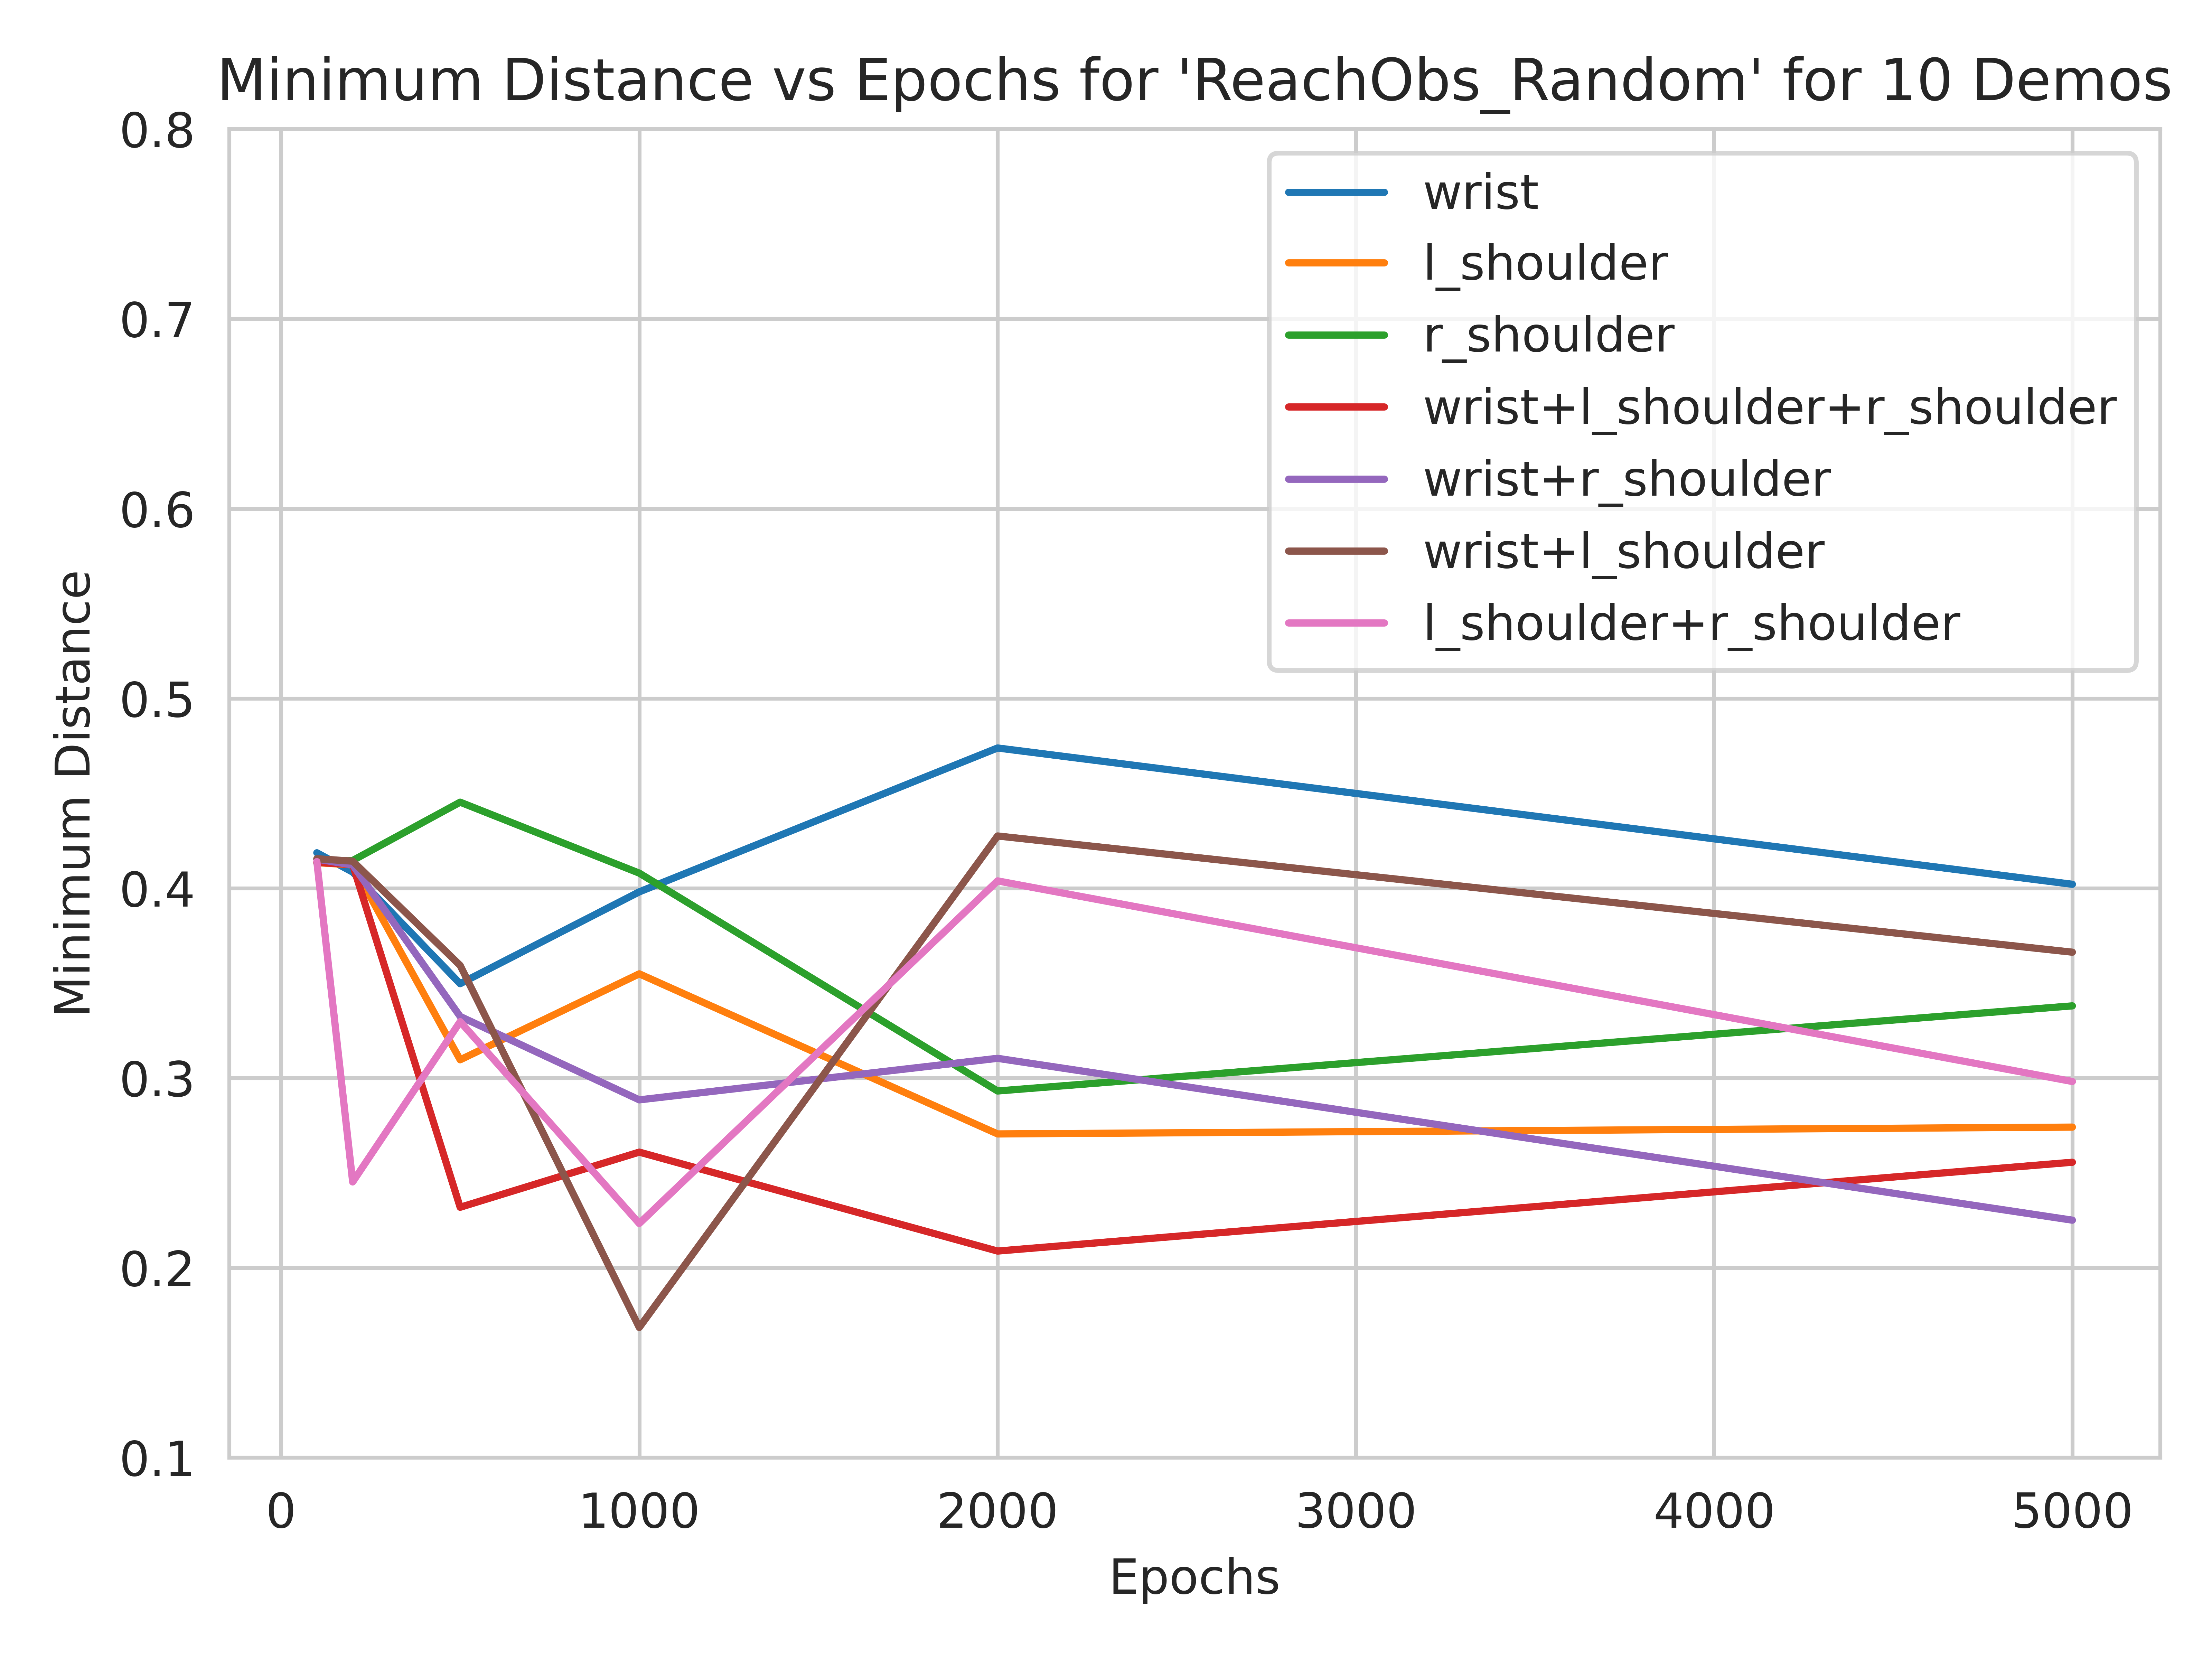
\includegraphics[width=\linewidth]{assets/cam-comb/reach-obs/ro_indrandom-obs-mindist-10demos.png}
    \caption{Minimum Distance to Target}\label{subfig:ro-indrandom-demo-mindist-10}
  \end{subfigure}
  \begin{subfigure}{0.45\linewidth}
    \centering
    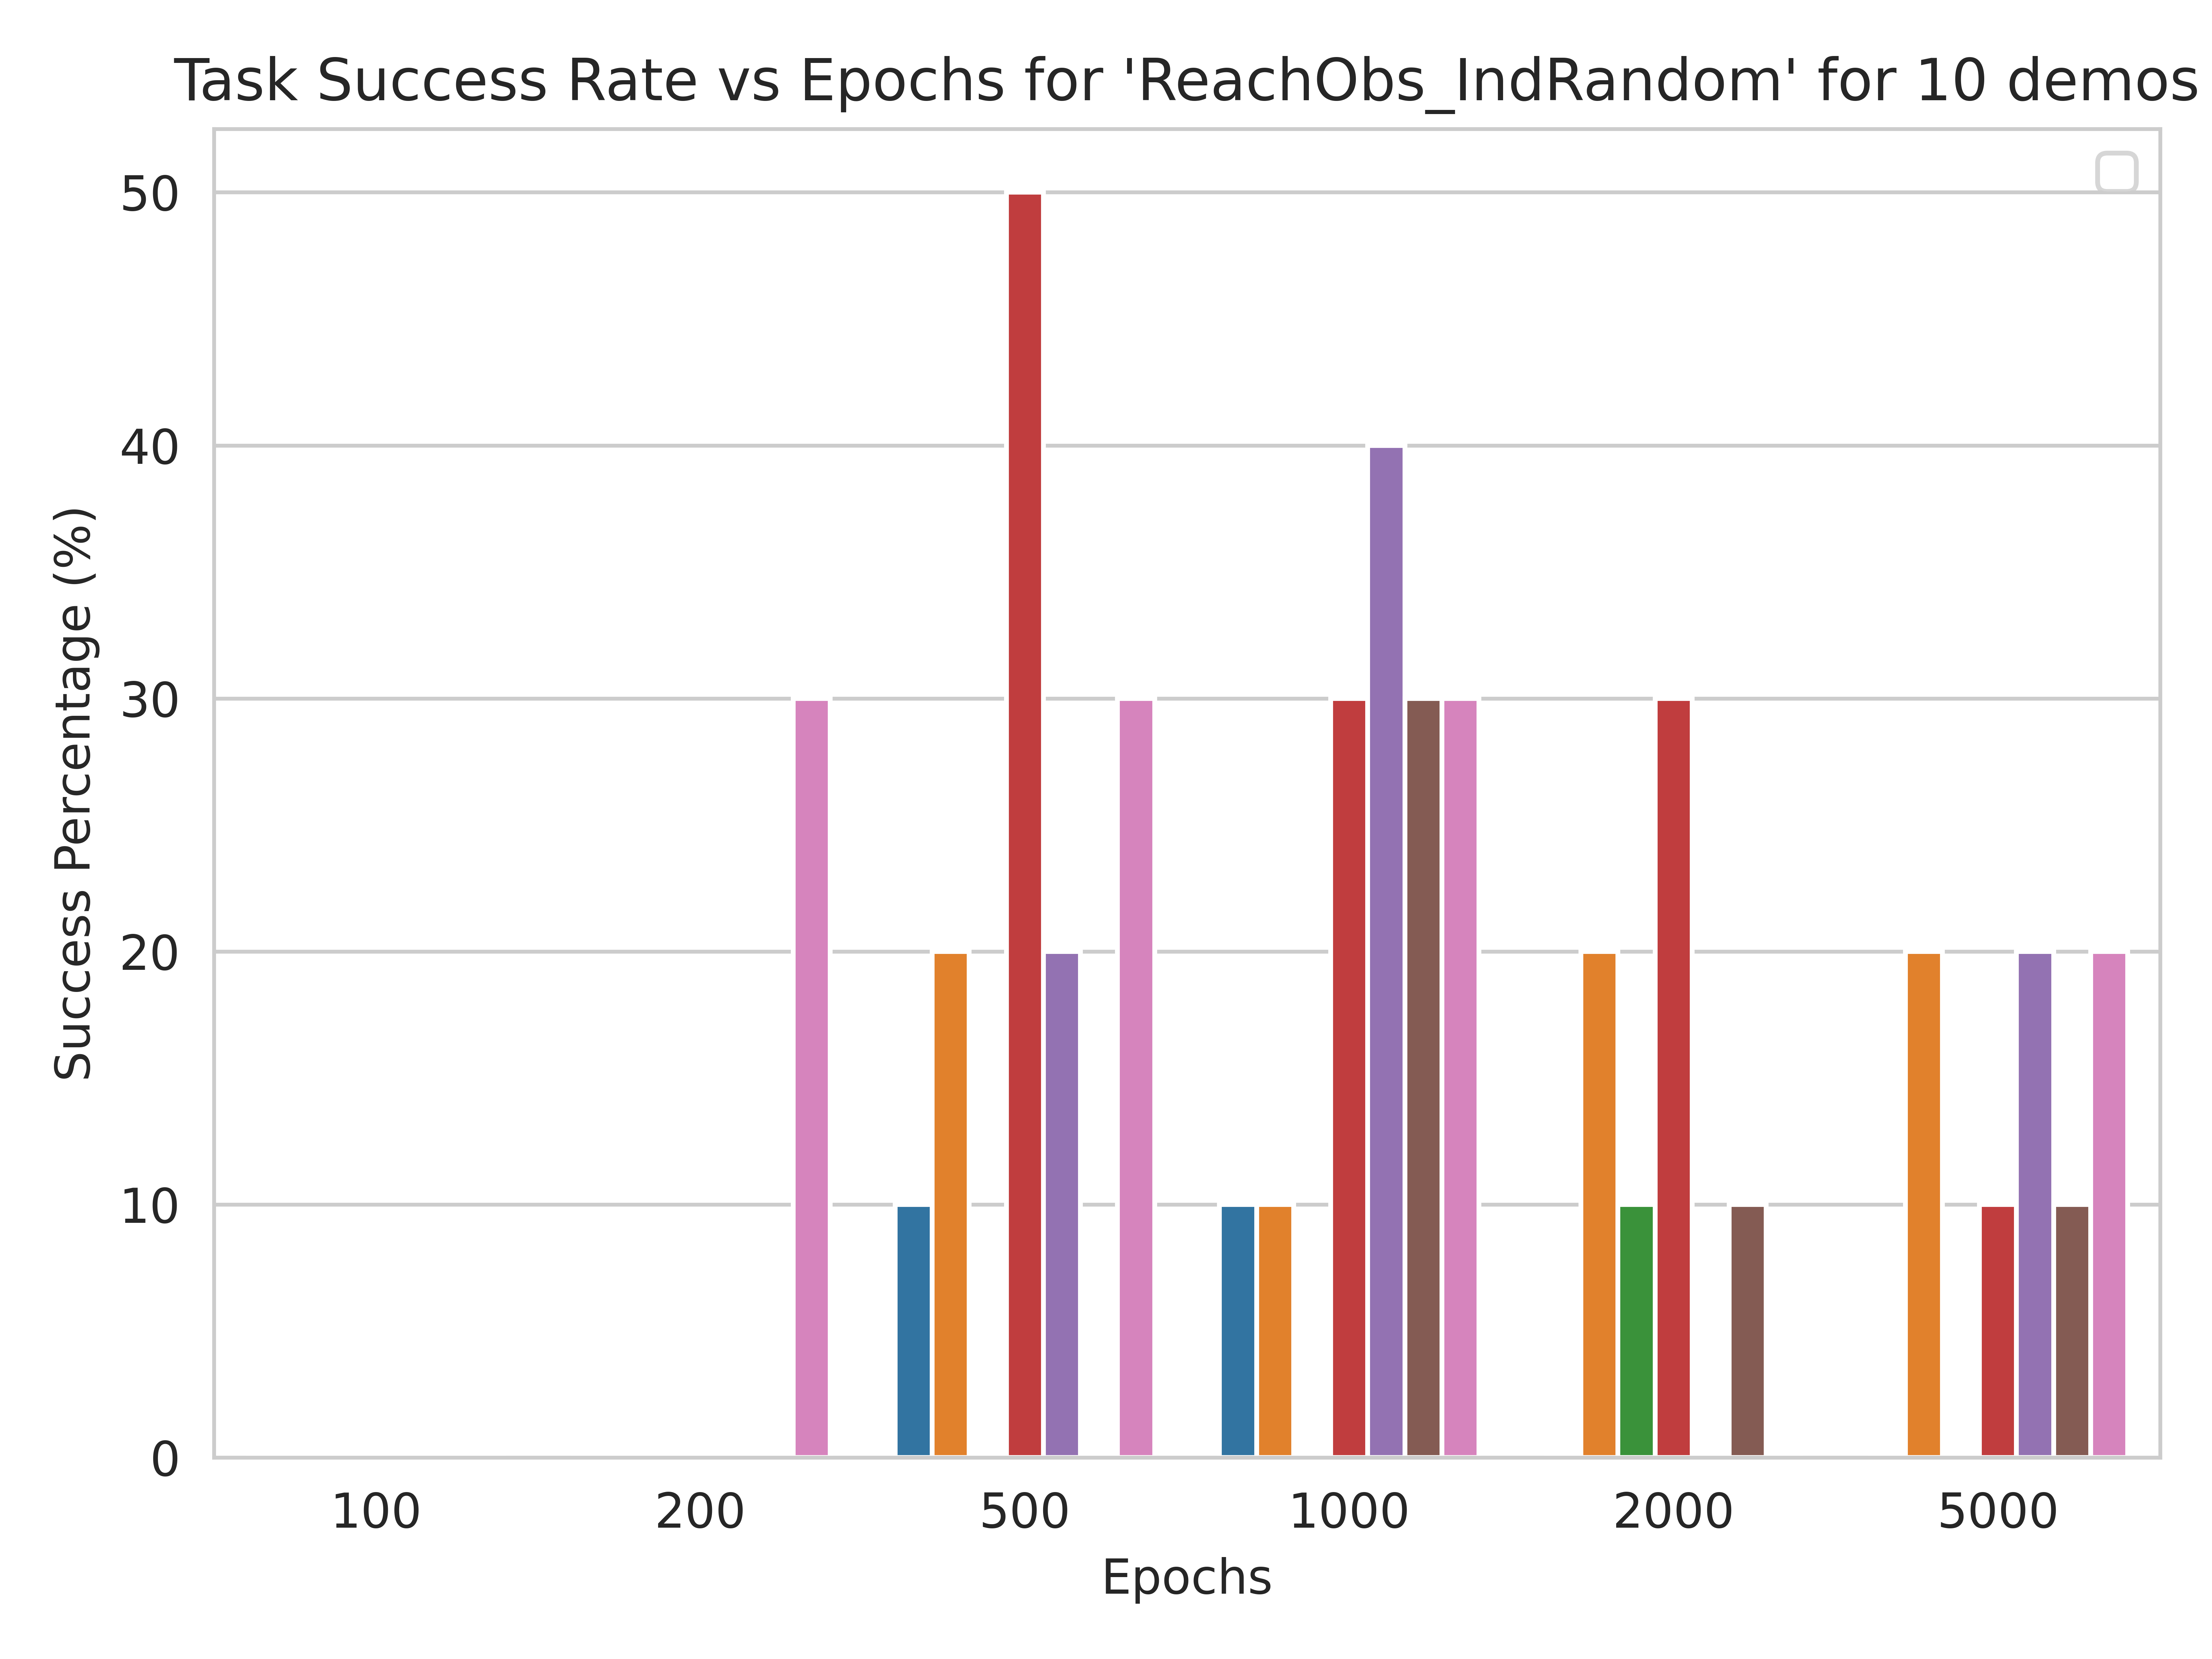
\includegraphics[width=\linewidth]{assets/cam-comb/reach-obs/ro_indrandom-demo-success-10demos.png}
    \caption{Success Rate (\%) of Task}\label{subfig:ro-indrandom-demo-success-10}
  \end{subfigure}
  \caption{Policy trained on 10 demos, using the \emph{demo dataset} from \ref{subsec:grasp-data-loading-changes}}\label{fig:ro-indrandom-demo-cams}
\end{figure}

\subsubsection{Dataset Differences}
I initially was planning on running the system with just the \emph{demo dataset}, however, one of the runs I accidentally included both. After reviewing the data, I realised the \emph{obs dataset} which prematurely flattens and forgets demo boundaries within the data seems to be performing better in this task; see \ref{subfig:ro-random-demo-success-10} and \ref{subfig:ro-random-obs-success-10}, more successes. Curiously though, the minimum distance to the target seems to be quite consistent, while the higher success, or course generally leads to a slightly smaller minimum distance.

My theory of why this happens is quite nuanced.\todo[color=purple]{} The \emph{obs dataset} here was trained using \verb|minibatch_size = 32|, the maximum episode length in these demos is $82$. This means that each epoch where the weights of the system are updated, we were exposing it to around one third of the data for a full episode. So, the first easy improvement is from extra training. The \emph{demo dataset} here was using a minibatch size of $1$, so for 10 demos, there is 10 updates per epoch, while the \emph{obs dataset} will do around $2.5$ more updates. 

The average episode for this task starts linearly getting near to the side of the obstacle, far away enough to not collide with it, then calculates a non-linear trajectory to curve inwards towards the target for the final bits of the movement.\todo[color=purple]{get a nice video of this for the presentation}. The non-linear part of the demo takes more steps than the linear part. Evident from the fully linear tasks like the grasp and the no obstacle reaching being around $40$ to $60$ steps. This means that the first $30$ ish steps are what the robot takes to move near the obstacle. Therefore, my running theory is that this system was performing better because the task was unintentionally compartmentalised into two sections. 1: Reaching to a side of the obstacle; and 2: Reaching towards the obstacle.

So, by unintentionally using this batch size we were updating the weights once to reach to a side of the obstacle then to the target. Finding this interesting, I ran more minibatch sizes to see if this was the case (see \todo{appendix ref}), although, this doesn't seem to be too important once the number of epochs increase, at lower epochs the success rate decreases across the board for larger batch sizes. Although, this is not conclusive, and it might not be ideal nitpicking every demo to specifically train each network, I thought this was an interesting property of sequential batching, even if there is no mechanism to explicitly take care of sequencing in the policy.

\begin{figure}[htpb] % htpb allows all placement
  \centering
  \begin{subfigure}{0.45\linewidth}
    \centering
    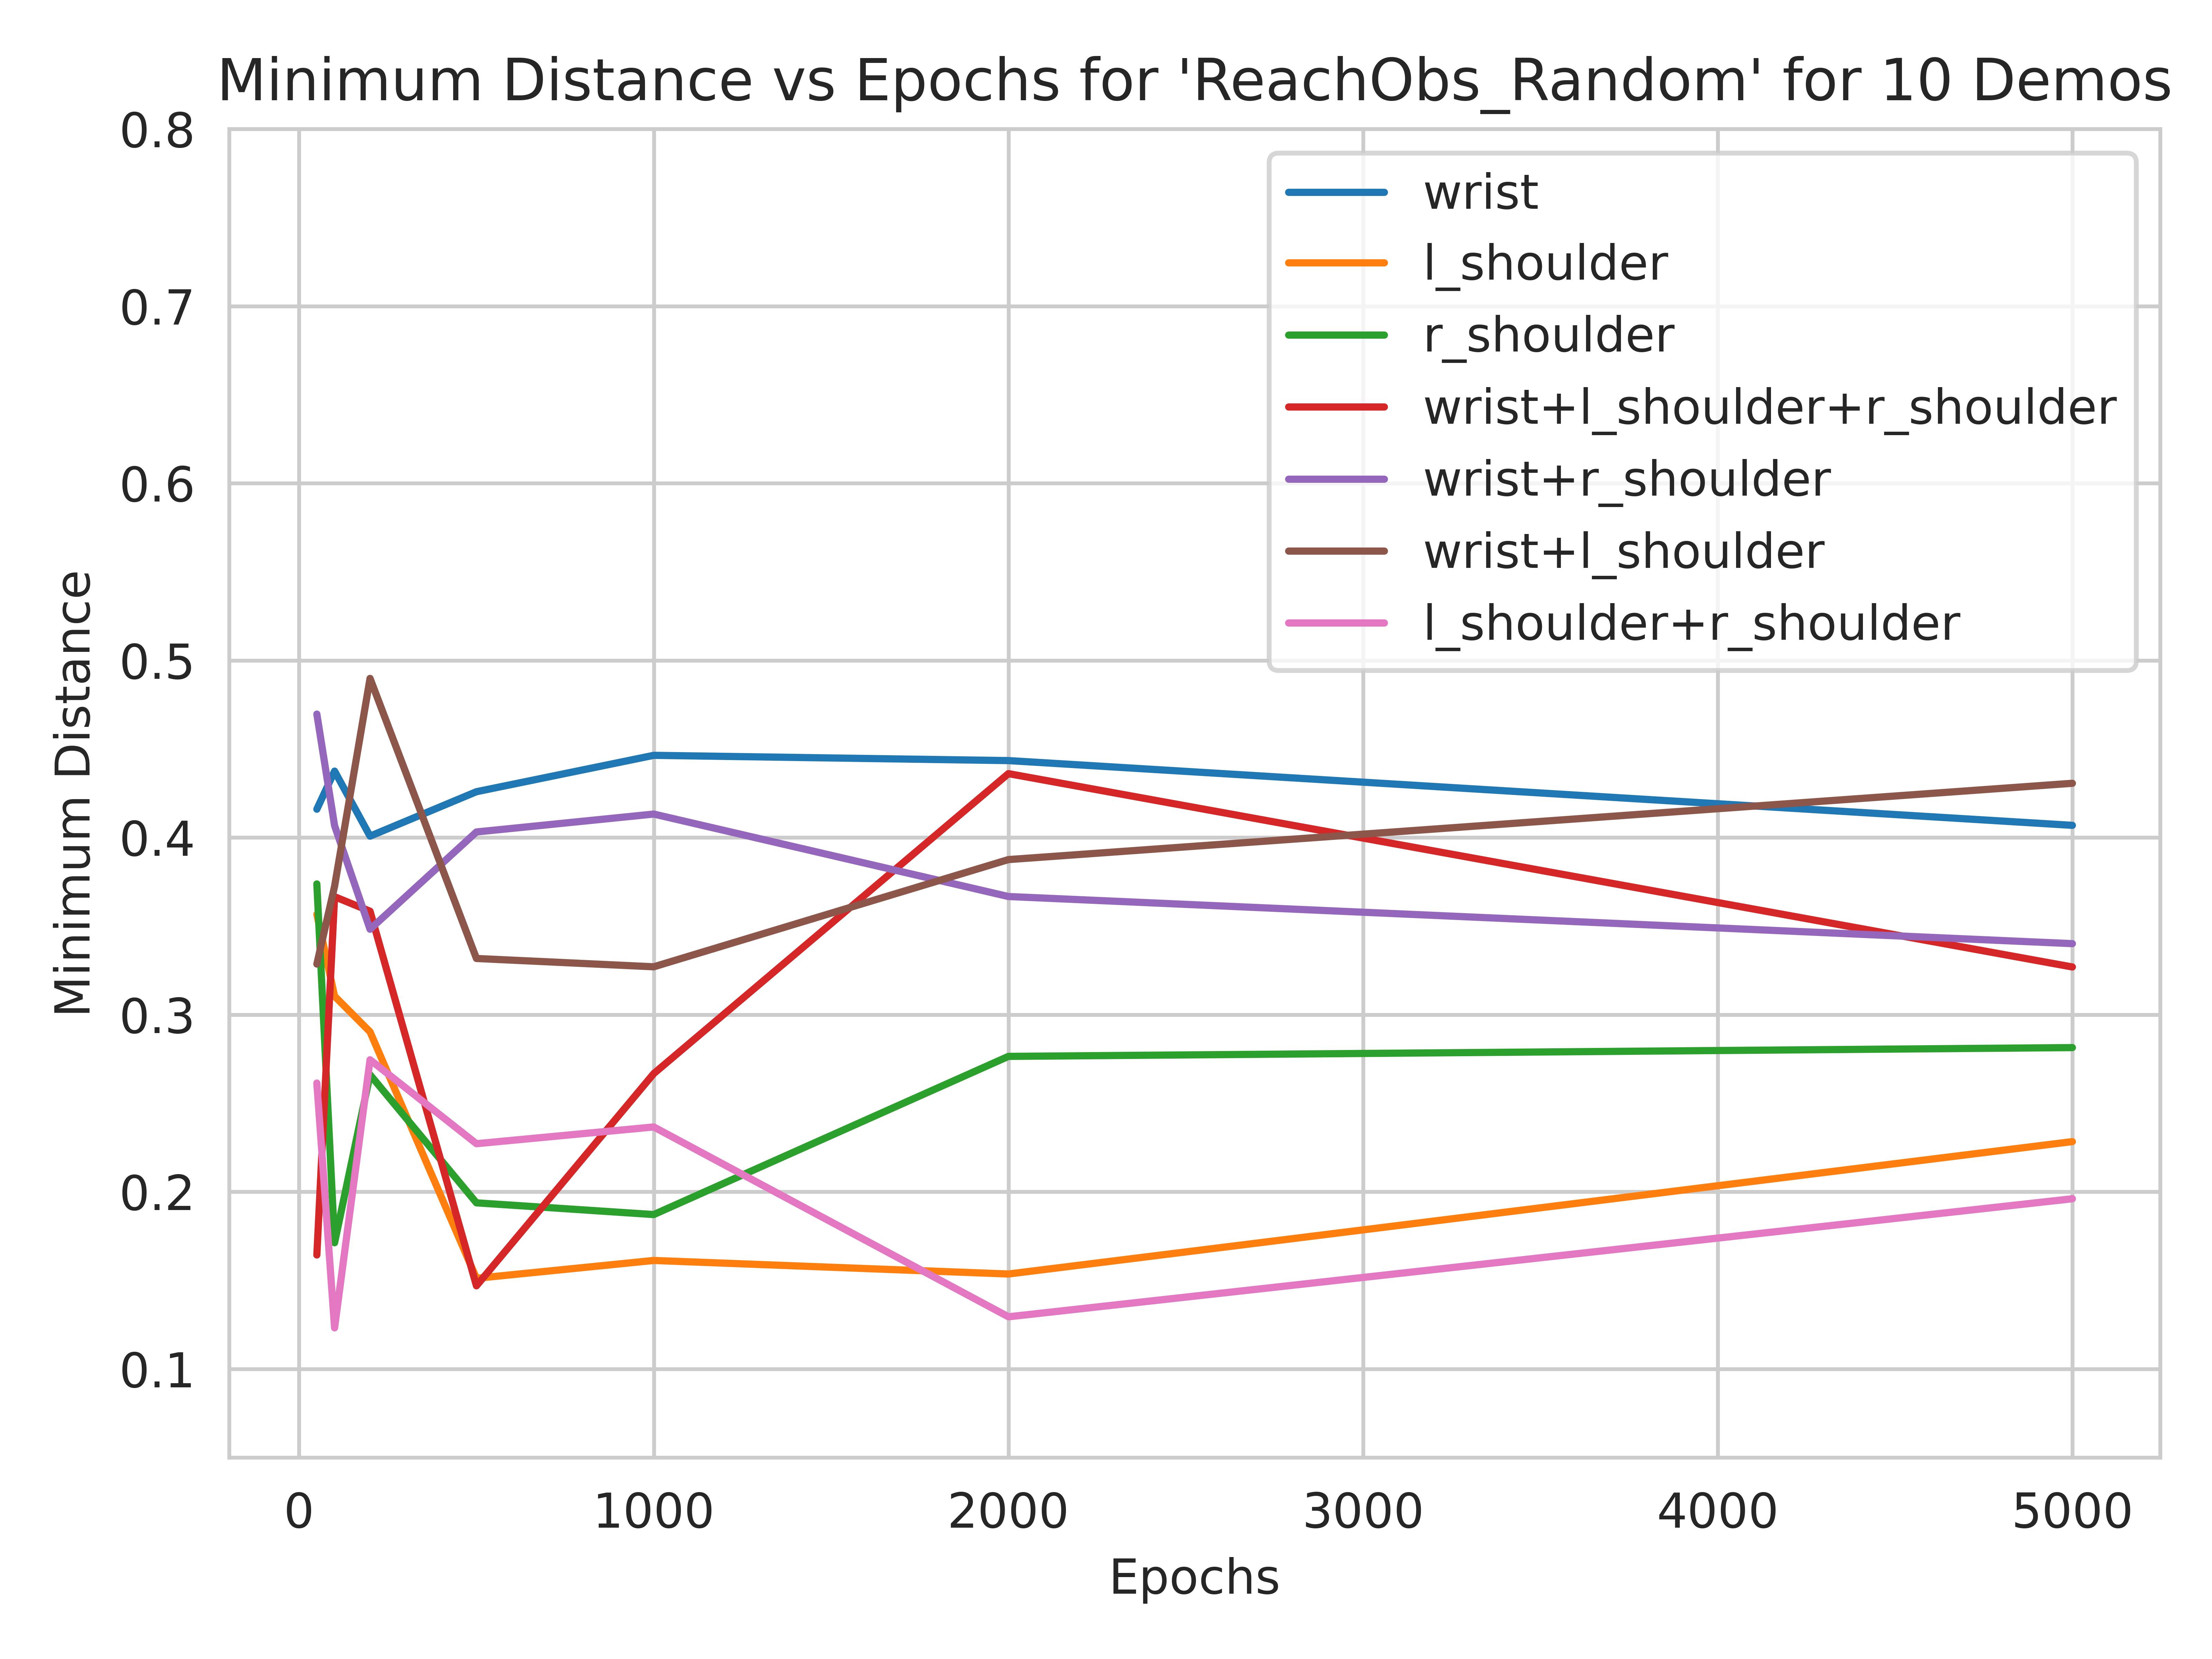
\includegraphics[width=\linewidth]{assets/cam-comb/reach-obs/ro_random-obs-mindist-10demos.png}
    \caption{Minimum Distance to Target}\label{subfig:ro-random-obs-dist-10}
  \end{subfigure}
  \begin{subfigure}{0.45\linewidth}
    \centering
    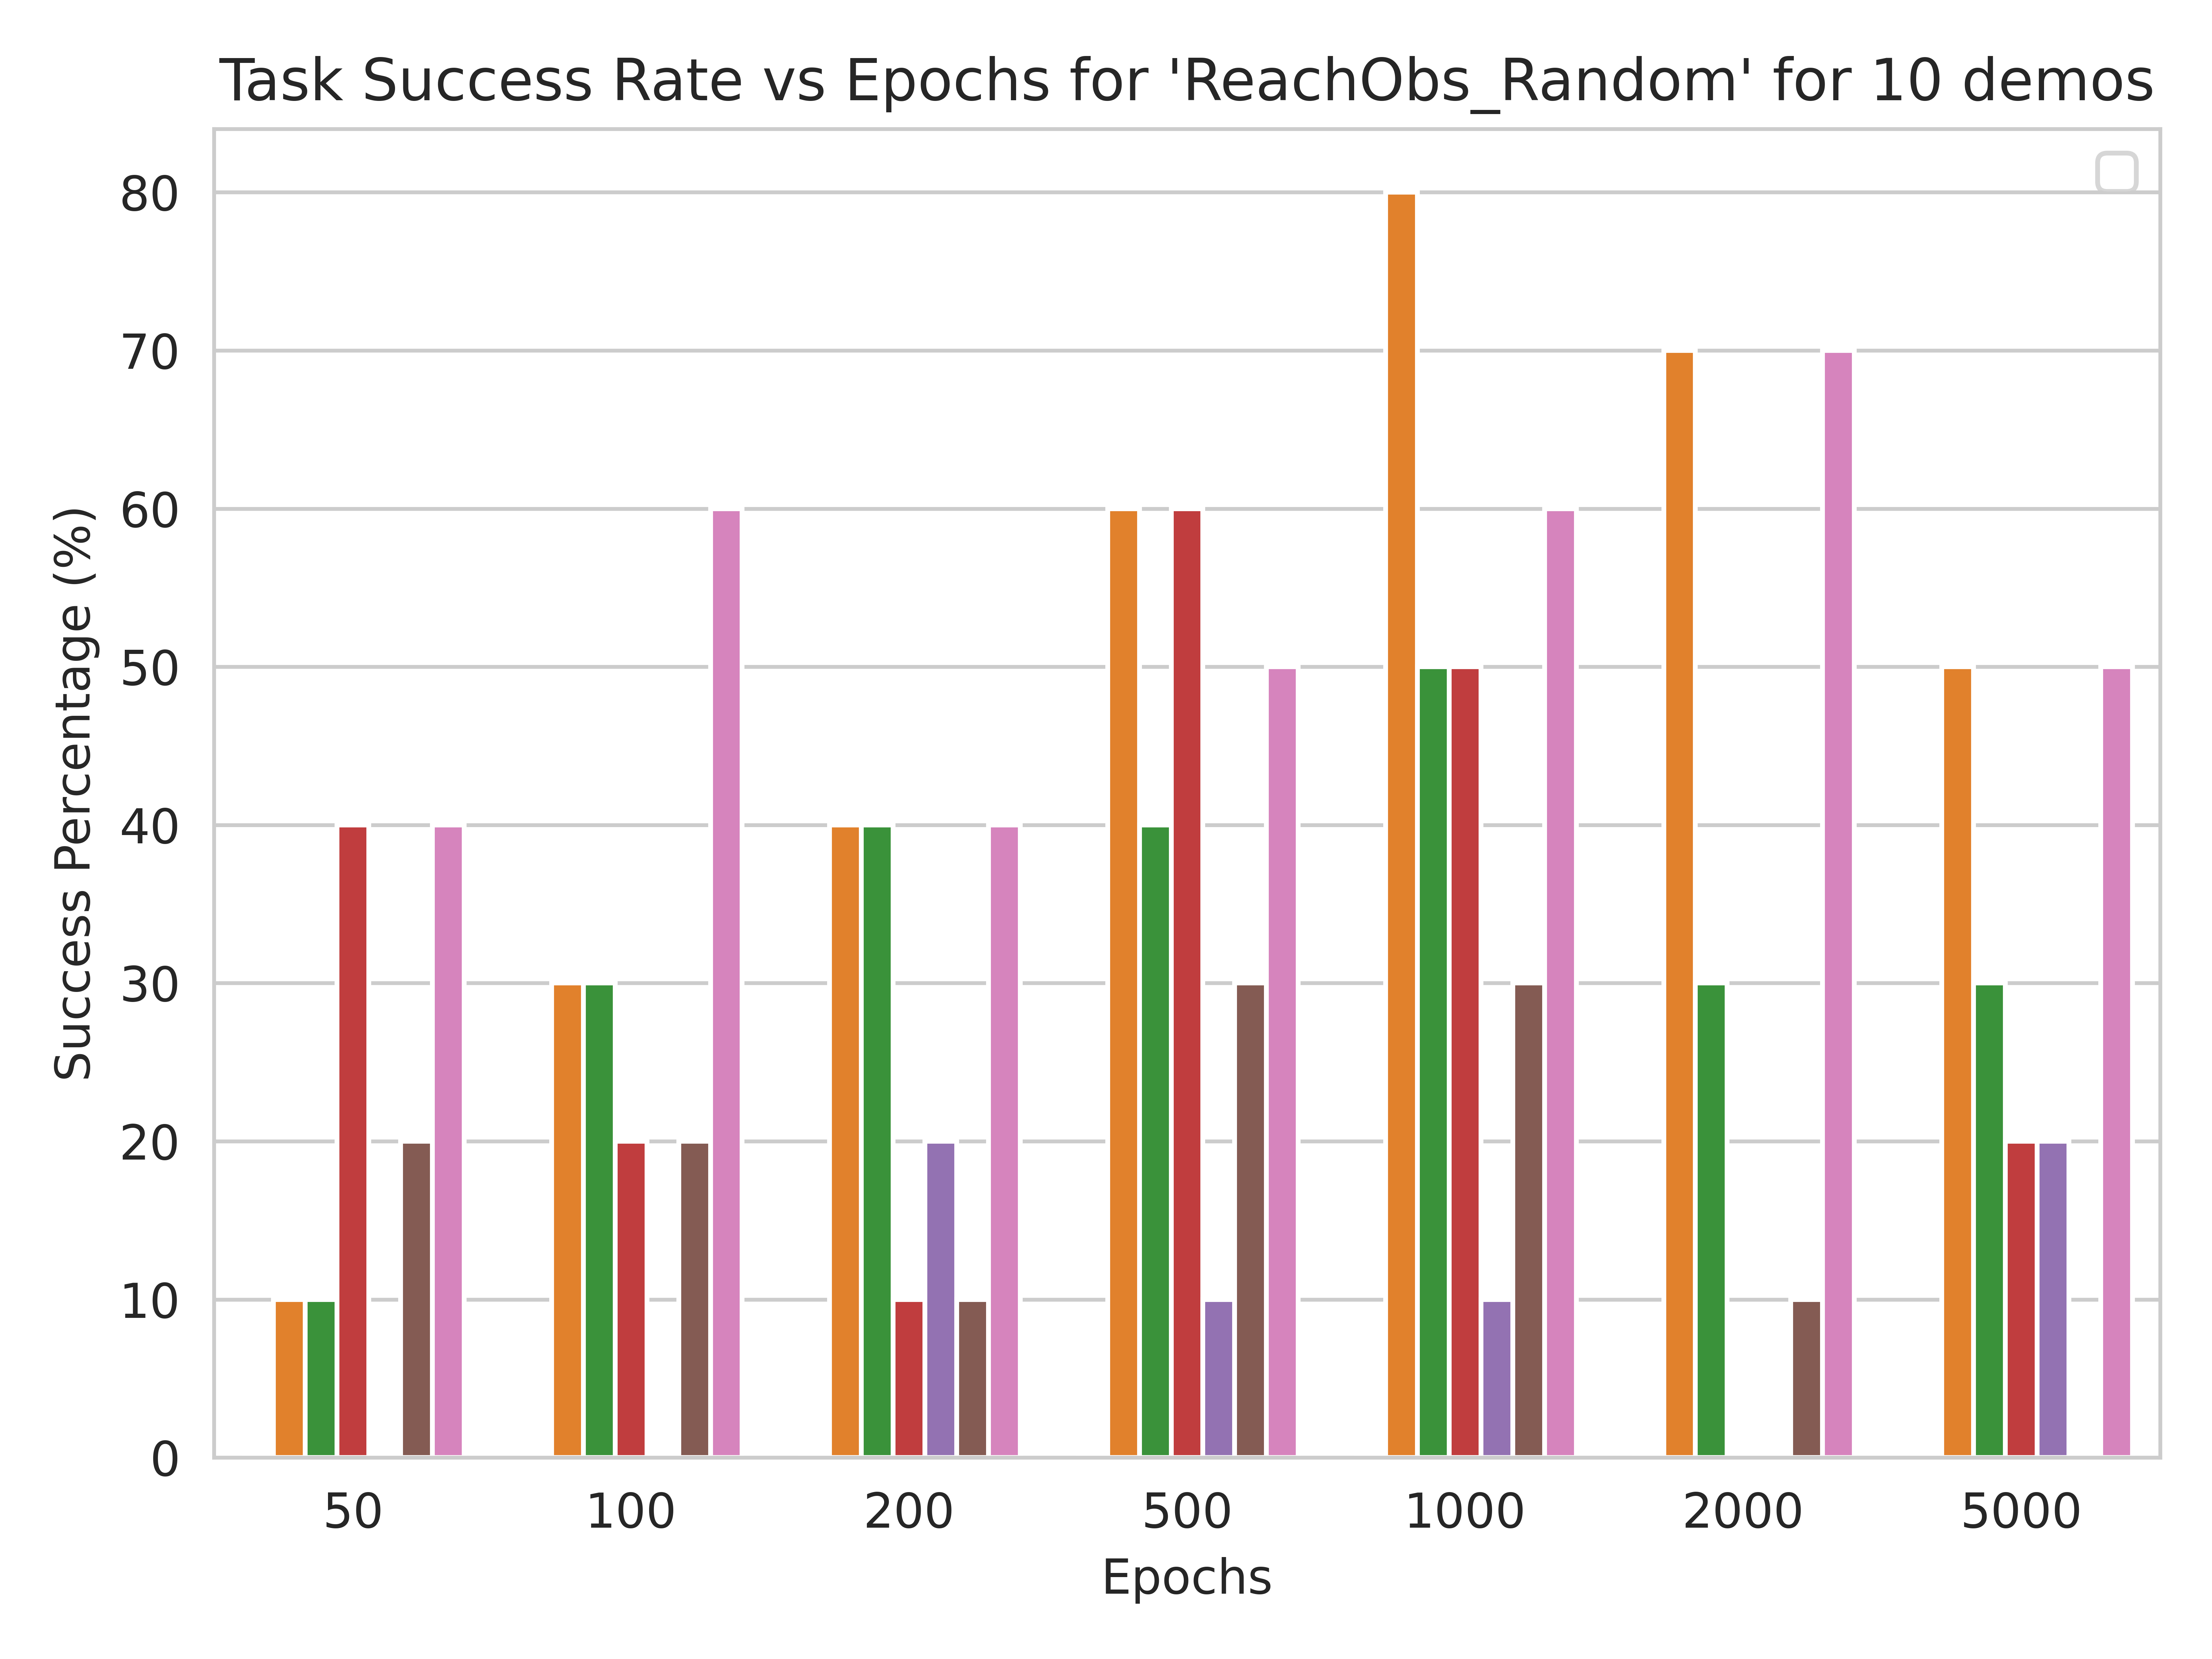
\includegraphics[width=\linewidth]{assets/cam-comb/reach-obs/ro_random-obs-success-10demos.png}
    \caption{Success Rate (\%) of Task}\label{subfig:ro-random-obs-success-10}
  \end{subfigure}
  \caption{Policy trained on 10 demos, using the \emph{obs dataset} from \ref{subsec:reach-data-loading}}\label{fig:ro-random-obs-cams}
\end{figure}

\subsubsection{Wrist Camera Alone isn't Enough}
Although, success rate graph looks nice at first glance, there is a distinct lack of blue; which is the wrist camera. Looking at the minimum distance the wrist achieves (around slightly less than$0.45$) we can see what it does a very good job of going around to the side of the obstacle (as the target is around $0.5$ metres from the obstacle), however, would struggle to make the last steps in touching the target. This is mostly due to the fact that the demonstrations are not necessarily pointing the wrist of the robot towards the target. This means all the wrist camera sees once it is past the obstacle is the table (a static view) which means it will likely likely get confused here and as there are no distinct features to latch onto, it will just execute a random movement it synthesised from the demos It was generally the case that the demo provided would take a wide swing around the obstacle, and almost every wrist rollout I managed to witness, it would just keep slinging the arm away -which is why the final distance graphs were very skewed.\todo[color=green]{link appendix graph} The wrist combined views were also prone to these, however sometimes the assisting camera would sometimes pick something up and course-correct.

Therefore, combining wrist and other cameras are almost always better as more coverage of the workspace guarantees less occlusions and more information the agent can work with to make decisions. Without a way to `look' towards the target the wrist camera alone is not going to cut it. Combining these ideas I moved onto the next section.

\section{Camera Attention Based on Colour}\label{sec:reach-obs-naive-cam-attn}
First idea bordering on `active vision' was to selectively accept the encoding from a single camera depending on what it was seeing. So, not necessarily looking around, but accepting the inputs from one of the cameras it has access to, guided by some prior information. This requires at least two camera views to `blend' otherwise given only one camera, it will act like the old policy.

The problem this is meant to fix is the policies involving wrist cameras tend to focus too much on wrist information when it is not relevant. As we can see in \ref{fig:ro-random-demo-cams}, these policies tend to sit above the $0.4$ min distance area which means they are continually hitting against the obstacle. The obstacle is around $0.39 \approx 0.43$ metres from the obstacle depending on its generation. So, if we can attend to different cameras depending on occlusion, we might be able to fix this problem.

\subsubsection{The Colour Score}
Given a set of RGB views (normalised to be  in range \(\left[0, 1\right]\)) I want to score them and weight them according to their perceived \emph{utility}, the first metric that comes to mind is colour. For every view, $\mathcal{V}_i$, $i$ representing different cameras and every pixel $\left( u, ~v\right)$ we calculate its euclidean distance to the target's colour: \( d_i\left(u, ~v\right) = ||\mathcal{V}_i\left(u, ~v\right) - t_{colour}||\), this is to guarantee the per-pixel score is a positive real number. 


Then to isolate our target colour I introduced two hyperparameters: \textbf{tolerance} and \textbf{softness}. Tolerance, $\varepsilon_{tol}$, defines the acceptable range of differences of what we can classify as the \emph{target colour}; red in this case. Softness, $\varepsilon_{sof}$, which helps adjust the harshness of sigmoid which we are feeding this for a signal. If softness is low the values within the tolerance will be a strong signal ($\approx 1$) and values without will be near $0$. 

So, the final classification of our score is defined as \(m_i\left(u, ~v\right) = \sigma \left(\left(\varepsilon_{tol} - d_i\left(u, ~v\right)\right)\times \varepsilon_{sof} \right)\) where \(\sigma\left(z\right) = \frac{1}{1 + e^{-z}}\): the sigmoid function. 
Then for scoring the image, I pool these tensors. Initially testing \emph{mean} pooling, \(\mathbf{S}_i = \max_{1<=u<=W, 1<=v<=H}m_i(i, ~v)\), which essentially acts as a signal of ``is the target colour in view or not?''. Then used \emph{mean} pooling \(\mathbf{S}_i = {\frac{1}{WH}\sum_{u = 1}^{W}\sum_{v = 1}^{H}m_i\left(u, ~v\right)} + c\) to give an overall visibility of the target within a view -adjusted by a constant. This will capture more nuanced inherent information about ``how much of the screen is the target?'' which is information about distance and occlusions.

The decision to use euclidean distance and sigmoid was to keep the colour score differentiable. This mainly helps in capturing the dynamics of the colour interaction within our neural network. A second benefit is, if I want to make the colour to be a learnable parameter we will be able to get the gradient of the loss with respect to ${RBG}_{target}$ to achieve this. Which can eliminate the colour prior.

\subsubsection{Scoring the Weighted Features}
When we have the score per view, we can weight the scores of each view against each other
\( \tilde{\mathbf{S}}_{i, x} = \frac{\mathbf{S}_{i, x}}{\sum_{}^{k \in v} \mathbf{S}_{i, k} + 10^{-6}} \); scalar term $10^{-6}$ being a numerical stabiliser and preventing vanishing gradients while not adding too much bias.

The features extracted from the cameras are concatenated with their respective score \( \begin{bmatrix} \mathbf{F}_i \\ \tilde{\mathbf{S}_i} \end{bmatrix} \in \mathbb{R}^{d + 1}\) where $d$ is the feature dimensions encoded after the conv layers. This, in turn, is fed into a attention network, to guess what the most important parts of the gives views are. Outputs of the network are then fed through a temperature scaled \emph{softmax}, \(sm\left(s\right)_i = \frac{e^{s_i / \mathcal{T}}}{\sum_{j \in v}{e^{s_j / \mathcal{T}}}}\). I also included temperature scaling here to introduce entropy in the resulting probability distribution across the views. This way the network will not be strongly attending on only one view.

\subsubsection{Encouraging Attention}
Final part of the puzzle is tuning the view scoring network. I calculated the attention predictions using KL divergence, \(D_{KL}\left(P ~||~ Q\right) = \sum_{x \in \mathcal{X}} P\left(x\right) \log \frac{P\left(x\right)}{Q\left(x\right)}\). This is a measure of the probability distribution difference\todo[color=green]{reference}. So, augmenting the loss of the overall network to be \(loss = loss_{action} + \lambda_{attn} D_{KL}\left( \hat{W}_{attn} ~||~ \mathbf{S}_i\right)\) where $\hat{W}_{attn}$ is the predicted weights, encouraging them to stay close to the ground truth scores.

\subsection{Feature Encoder Coupling}
Final proposition for this network is to check whether disconnecting the feature encoders makes a difference. In theory, every view having its own feature extractor might allow the network to learn inherent pose and view information for that specific view. For example, the shoulder cameras.  Although, following the same logic, keeping a joint extractor might allow to policy to learn how different poses and information from those poses interact in tandem. As the workspace and hence the observations are quite similar.

